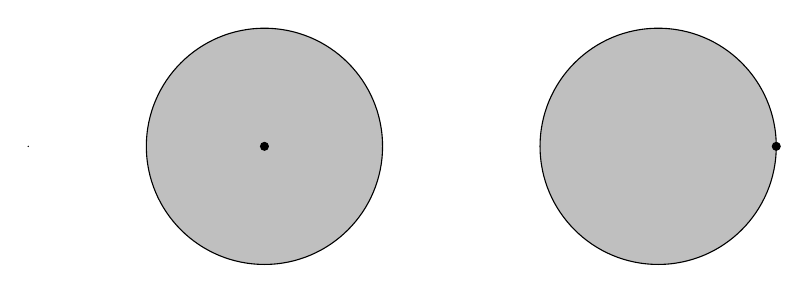
\begin{tikzpicture}
\draw (0,0) circle(0.00001cm);
\filldraw[fill = lightgray, draw = black] (3,0) circle (1.5cm);
\filldraw (3,0) circle (0.05cm);
\filldraw[fill = lightgray, draw = black] (8,0) circle (1.5cm);
\filldraw (9.5,0) circle (0.05cm);
\end{tikzpicture}
\newline

The concept of moment of inertia causes quite a good deal of trouble for many people because it is not something we can get an intuitive feel for and because it gets complex when we move beyond the most simple examples. However, if we clearly define the purpose of using the moment of inertia, it should make things much easier. Simply put, the moment of inertia is analogous to mass in linear motion. The larger the moment of inertia of an object, the “harder” it will be to accelerate it rotationally(and keep it going at a constant velocity when we have friction, as we will soon see, it will have units of $$kg \cdot m^2$$ Moments of Inertia are also confusing because their value is not only tied to the shape and size of the object, but also the axis around which the object in question is being rotated. To understand the need for the moment of inertia we first need to talk about angular momentum. Angular momentum is the momentum objects will have from rotating rather than from moving linearly. For a point mass, momentum $\vec{p}$ is equal to $m\vec{v}$. Angular momentum will be analogous to this. The analogy for $m$ will be I, and the analogy for velocity will be angular velocity, $\omega$. The symbol we normally use for angular momentum is $\vec{L}$ and in the right circumstances, is equal to $$I\omega$$ However, the true definition of the angular momentum of something about a point is $\vec{r} \times \vec{p}$. We assume that when we have rigid body motion, the object will be rotating about a certain point in circular fashion, so \begin{equation}\vec{r} \times \vec{p} = rp = mrv\end{equation} However, we have said that this is equal to $I\omega$. So we have that $$I\omega=mrv=mr^2\omega$$ so $I=mr^2$. This formula is only for a point mass rotating in a circle of radius r as part of a rigid body. It will not work when we have entire rigid bodies that are rotating. When we do this, we will talk about small masses, and tiny incremental moments of inertia, so we write that $dI=r^2 dm$. This is not anything new, but it will allow us to integrate over areas with changing radius or mass density to solve our problems. 

For example, let us first take the example of a perfectly flat frisbee(so we can ignore the third dimension) with surface density $\sigma$. This means that the mass of any region of the frisbee divided by that area is equal to $\sigma$. So, therefore the mass of the total frisbee is $$\pi r^2 \sigma$$ Now, we will use a sort of trick. We are to try to find the total moment of inertia of the frisbee by integrating over circles of different radii from 1 to r. We know that the mass of a circle of radius $r$ in general is $M=\sigma \pi r^2$. So, we can differentiate both sides of the equation with respect to r to find that \begin{equation}dM= 2\pi r \sigma dr\end{equation} This means that the mass of the little extra piece of a circle of radius $r+dr$ approaches $2\pi r \sigma dr$ as $dr$ goes to 0. I challenge you to find this yourself just using geometry. Well, we now have our expression for $dM$ as a function of the radius of the circle so we can integrate to find the moment of inertia. We have that $I= \int_{0}^{r} 2\pi r^3 \sigma \ dr$. We integrate from $0$ to $r$ because we are finding the mass of the little masses of circles from $0$ to $r$. When we integrate we find our expression is equal to $$\frac{\pi \sigma}{2} \cdot r^4$$ But $\sigma \pi r^2$ is equal to the mass of the frisbee, so the moment of inertia is $I = \frac{mr^2}{2}$. Now, this was a special example where we were rotating the frisbee about an axis parallel to its center of mass. However, often things will not rotate about their center of mass. It would be quite difficult to use our formula for the moment of inertia above when we are rotating about an axis not parallel to the center of mass. The integrals can get quite messy, and it is much easier to use the so-called parallel axis theorem. The parallel axis theorem states that the moment of inertia of a rigid body about an axis other than one parallel to the center of mass is equal to the moment of inertia about the center of mass, plus the mass of the object times the distance from the axis of rotation to the axis along the center of mass squared. In symbols, this is often written as \begin{equation}I=I_cm+mr^2\end{equation} I challenge you to use this formula to find the moment of inertia of a frisbee about its outer edge. Lastly, I challenge you to find the moments of inertia of a normal cylinder, a hollow cylinder, a sphere(this one is very tricky), and of a square about its center, a flat rod. You can assume you know both the mass of the item and the radius or length of it. We will see how important these are later, however, deriving them is mostly math and not physics, so they will not be covered here. In practice, you will often be able to look these up in a book. Lastly, it might be important for you to consider the moment of inertia of objects with holes. Although they do not appear on the AP Exam, the simple answer is that you can find the moment of inertia of objects with holes by imaging the hole wasn’t there and finding the moment of inertia, and then just finding the moment of inertia of what would be the mass of the hole, and then subtracting the second quantity from the first. Neat!